\documentclass[../main]{subfiles}

\pgfplotsset{every axis/.append style={
                    axis x line=middle,    % put the x axis in the middle
                    axis y line=middle,    % put the y axis in the middle
                    axis line style={<->}, % arrows on the axis
                    xlabel={$Re(z)$},          % default put x on x-axis
                    ylabel={$Im(z)$},          % default put y on y-axis
                    }}
\tikzset{>=stealth}

\begin{document}

\section{Complex Numbers}

\subsection{Imaginary Numbers}
	\begin{equation*} \begin{gathered}
		i = \sqrt{-1} \\
		i^2 = -1 \\
		i^4 = i^2 \times i^2 = 1
	\end{gathered} \end{equation*}

\subsection{Cartesian Representation}

	\subsubsection{Complex Numbers}
	Complex numbers are written in the form:
	\begin{equation*} \begin{gathered}
		z = a + ib \quad a,b \in \mathbb{R} \\
		\text{Where} \quad Re(z) = a \quad Im(z) = b
	\end{gathered} \end{equation*}
	And populate the set \(\mathbb{C}\)
	\subsubsection{Conjugates}
	\begin{equation*} \begin{gathered}
		\text{For} \quad w = a+ib \quad z = c+id \\
		w^* = a - ib \\
		ww^* = a^2 + b^2 = |w|^2\\
		(w+z)^* = w^* + z^* \\
		(wz)^* = w^*z^* \\
	\end{gathered} \end{equation*}
	\subsubsection{Algebraic Manipulation}  
	\begin{equation*} \begin{gathered}
		\text{For} \quad w = a+ib \quad z = c+id \\
		w = z \implies a = c, b = d \quad \text{\bf{IMPT}} \\
		w + z = (a+c) + i(b+d) \\
		w - z = (a-c) + i(b-d) \\
		w * z = (ac-bd) + i(ad+bc) \\
		|w| = \sqrt{a^2+b^2} \\
		\sqrt{w} \quad \text{occurs with a \(\pm\) sign}
	\end{gathered} \end{equation*}
	For division, remove \(i\) from denominator by multiplying numerator and denominator by conjugate and then solve:
	\begin{equation*} \begin{split}
		\frac{w}{z} & = \frac{w}{z} \times \frac{z^*}{z^*} \\
					& = \frac{wz^*}{zz^*} \\
					& = \frac{wz^*}{c^2+d^2}
	\end{split} \end{equation*}

\subsection{Complex Polynomial Roots}
	
	\subsubsection{Fundamental Theorem of Algebra}
	A polynomial of degree \(n\) has \(n\) real or complex roots. 

	\subsubsection{Finding Complex Roots}
	If a polynomial has all real coefficients, complex roots occur in conjugate pairs. Write as such in exams:
	
	\[ f(x) \quad \text{has real coefficients} \]
	\[ a+ib \quad \text{is a root} \implies a-ib \quad \text{is a root} \] 

	For a polynomial with complex coefficients, use quadratic general formula. Note that a \(\pm\) will still be present somewhere.

\subsection{Polar Representation}
	
	\subsubsection{Polar Representation}
	\begin{equation*} \begin{gathered}
		z = re^{i\theta} \quad r \in \mathbb{R}^{+}_0 \quad -\pi < \theta \leq \pi \\
		|z| = r \quad arg(z) = \theta = \tan^{-1}(\frac{a}{b}) \\
		Re(z) = r\cos(\theta) \\ Im(z) = r\sin(\theta) \\
		re^{i\pi} = -1 \quad re^{i0} = 1 \\
		re^{i\frac{\pi}{2}} = i \quad re^{i\frac{-\pi}{2}} = -i
	\end{gathered} \end{equation*}
	\subsubsection{Algebraic Manipulation}
	\begin{equation*} \begin{gathered}
		\text{For} \quad z_1 = r_1e^{i\theta_1} \quad z_2 = r_2e^{i\theta_2} \\
		z_1z_2 = r_1r_2 e^{i(\theta_1+\theta_2)} \\
		\frac{z_1}{z_2} = \frac{r_1}{r_2} e^{i(\theta_1-\theta_2)} \\
		z_1^n = r_1^n e^{in\theta_1} \\
		\sqrt{z_1} = \sqrt{r_1} e^{i(\frac{\theta_1}{2})}, \sqrt{r_1} e^{i(\frac{\theta_1}{2}+\pi)}
	\end{gathered} \end{equation*}

\subsection{Geometric Representation}
	
	\subsubsection{Argand Diagrams}
	Cartesian form describes the x and y coordinate on the real and imaginary axis. \\
	Polar form describes the distance between the point and the origin as well as the angle a line from the point to the origin makes with the positive real axis. \\
	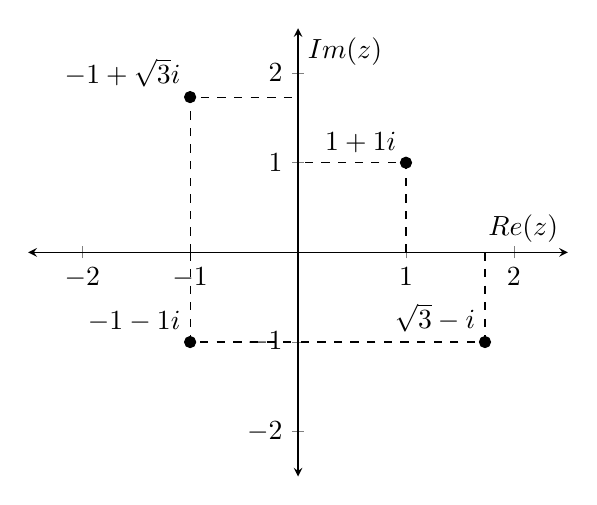
\begin{tikzpicture} \begin{axis}[xmin=-2.5,xmax=2.5,ymin=-2.5,ymax=2.5,samples=100,mark=none,smooth]
		\addplot [black, mark=*, mark options={draw=black}, only marks] coordinates {(1,1)}
			node [anchor=south east] {$1+1i$};
		\draw[dashed] (axis cs:1,0) -- node{} (axis cs:1,1) -- node{} (axis cs:0,1);
		\addplot [black, mark=*, mark options={draw=black}, only marks] coordinates {(-1,-1)}
			node [anchor=south east] {$-1-1i$};
		\draw[dashed] (axis cs:-1,0) -- node{} (axis cs:-1,-1) -- node{} (axis cs:0,-1);
		\addplot [black, mark=*, mark options={draw=black}, only marks] coordinates {(-1,1.732)}
			node [anchor=south east] {$-1+\sqrt{3}i$};
		\draw[dashed] (axis cs:-1,0) -- node{} (axis cs:-1,1.732) -- node{} (axis cs:0,1.732);
		\addplot [black, mark=*, mark options={draw=black}, only marks] coordinates {(1.732,-1)}
			node [anchor=south east] {$\sqrt{3}-i$};
		\draw[dashed] (axis cs:1.732,0) -- node{} (axis cs:1.732,-1) -- node{} (axis cs:0,-1);
	\end{axis} \end{tikzpicture}
	\\
	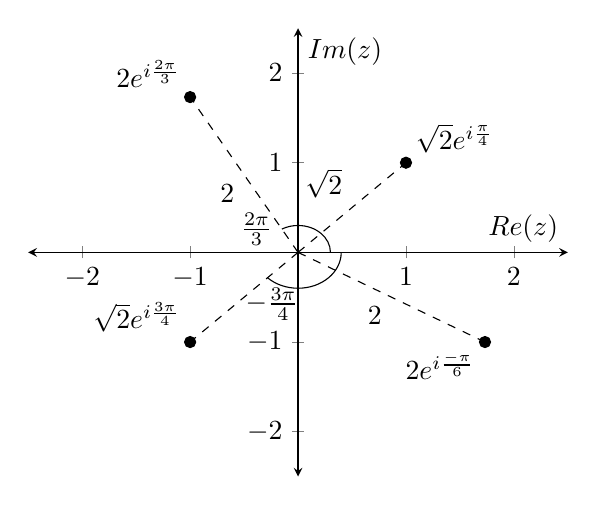
\begin{tikzpicture} \begin{axis}[xmin=-2.5,xmax=2.5,ymin=-2.5,ymax=2.5,samples=100,mark=none,smooth]
		\addplot [black, mark=*, mark options={draw=black}, only marks] coordinates {(1,1)}
			node [anchor=south west] {$\sqrt{2}e^{i\frac{\pi}{4}}$};
		\draw[dashed] (axis cs:0,0) -- node[anchor=south east]{$\sqrt{2}$} (axis cs:1,1);
		\addplot [black, mark=*, mark options={draw=black}, only marks] coordinates {(-1,-1)}
			node [anchor=south east] {$\sqrt{2}e^{i\frac{3\pi}{4}}$};
		\draw[dashed] (axis cs:0,0) -- node[anchor=west]{} (axis cs:-1,-1);
		\addplot [black, mark=*, mark options={draw=black}, only marks] coordinates {(-1,1.732)}
			node [anchor=south east] {$2e^{i\frac{2\pi}{3}}$};
		\draw[dashed] (axis cs:0,0) -- node[anchor=north east]{$2$} (axis cs:-1,1.732);
		\addplot [black, mark=*, mark options={draw=black}, only marks] coordinates {(1.732,-1)}
			node [anchor=north east] {$2e^{i\frac{-\pi}{6}}$};
		\draw[dashed] (axis cs:0,0) -- node[anchor=north east]{$2$} (axis cs:1.732,-1);
		\draw (axis cs:0.3,0) arc [radius=0.3,start angle = 0, end angle = 120] node[anchor=east]{$\frac{2\pi}{3}$};
		\draw (axis cs:0.4,0) arc [radius=0.4,start angle = 0, end angle = -135] node[anchor=100]{$-\frac{3\pi}{4}$};
	\end{axis} \end{tikzpicture}
	\subsubsection{Geometric Manipulation}
	Multiplying by \(re^{i\theta}\) scales the number by a factor of \(r\) and rotates anticlockwise by an angle of \(\theta\) about the origin. \\
	Multiplying by \(i\) rotates a complex number by \(\frac{\pi}{2}\), or \(90\degree\) anticlockwise. \\
	The conjugate of a complex number is a reflection of the complex number on the x axis.


\end{document}